%%%%%%%%%%%%%%%%%%%%%%%%%%%%%%%%%%%%%
%                                   %
% Compile with XeLaTeX and biber    %
%                                   %
% Questions or comments:            %
%                                   %
% joshua dot mcneill at uga dot edu %
%                                   %
%%%%%%%%%%%%%%%%%%%%%%%%%%%%%%%%%%%%%

\documentclass{beamer}
  % Read in standard preamble (cosmetic stuff)
  %%%%%%%%%%%%%%%%%%%%%%%%%%%%%%%%%%%%%%%%%%%%%%%%%%%%%%%%%%%%%%%%
% This is a standard preamble used in for all slide documents. %
% It basically contains cosmetic settings.                     %
%                                                              %
% Joshua McNeill                                               %
% joshua dot mcneill at uga dot edu                            %
%%%%%%%%%%%%%%%%%%%%%%%%%%%%%%%%%%%%%%%%%%%%%%%%%%%%%%%%%%%%%%%%

% Beamer settings
% \usetheme{Berkeley}
\usetheme{CambridgeUS}
% \usecolortheme{dove}
% \usecolortheme{rose}
\usecolortheme{seagull}
\usefonttheme{professionalfonts}
\usefonttheme{serif}
\setbeamertemplate{bibliography item}{}

% Packages and settings
\usepackage{fontspec}
  \setmainfont{Charis SIL}
\usepackage{hyperref}
  \hypersetup{colorlinks=true,
              allcolors=blue}
\usepackage{graphicx}
  \graphicspath{{../../figures/}}
\usepackage[normalem]{ulem}
\usepackage{enumerate}

% Document information
\author{M. McNeill}
\title[FREN2001]{Français 2001}
\institute{\url{joshua.mcneill@uga.edu}}
\date{}

%% Custom commands
% Lexical items
\newcommand{\lexi}[1]{\textit{#1}}
% Gloss
\newcommand{\gloss}[1]{`#1'}
\newcommand{\tinygloss}[1]{{\tiny`#1'}}
% Orthographic representations
\newcommand{\orth}[1]{$\langle$#1$\rangle$}
% Utterances (pragmatics)
\newcommand{\uttr}[1]{`#1'}
% Sentences (pragmatics)
\newcommand{\sent}[1]{\textit{#1}}
% Base dir for definitions
\newcommand{\defs}{../definitions}


  % Packages and settings
  \usepackage{phonrule}
  \usepackage[style=apa, backend=biber]{biblatex}
    \addbibresource{../references/References.bib}

  % Document information
  \subtitle[Variation at Different Levels]{Variation at Different Levels of Linguistic Structure}

  %% Custom commands
  % Subsection/frame titles
  \newcommand{\suboneone}{Which levels?}
  \newcommand{\subonetwo}{Phonetics}
  \newcommand{\subonethree}{Phonology}
  \newcommand{\subonefour}{Morphology}
  \newcommand{\subonefive}{Syntax}
  \newcommand{\subonesix}{Semantics and lexicons}
  \newcommand{\suboneseven}{Practice}

\begin{document}
  % Read in the standard intro slides (title page and table of contents)
  %%%%%%%%%%%%%%%%%%%%%%%%%%%%%%%%%%%%%%%%%%%%%%%%%%%%%%%%%%%%%%%%
% This is a standard set of intro slides used in for all slide %
% documents. It basically contains the title page and table of %
% contents.                                                    %
%                                                              %
% Joshua McNeill                                               %
% joshua dot mcneill at uga dot edu                            %
%%%%%%%%%%%%%%%%%%%%%%%%%%%%%%%%%%%%%%%%%%%%%%%%%%%%%%%%%%%%%%%%

\begin{frame}
  \titlepage
  \tiny{Office: % Basically a variable for office hours location
Gilbert 121\\
        Office hours: % Basically a variable for office hours
 lundi, mercredi, vendredi 10:10--11:10
}
\end{frame}

\begin{frame}
  \tableofcontents[hideallsubsections]
\end{frame}

\AtBeginSection[]{
  \begin{frame}
    \tableofcontents[currentsection,
                     hideallsubsections]
  \end{frame}
}


  \section{Variation at Different Levels}
    \subsection{\suboneone}
      \begin{frame}{\suboneone}
        \begin{block}{Language variation can occur at any level}
          \begin{itemize}
            \item Phonetics
            \item Phonology
            \item Morphology
            \item Syntax
            \item Semantics (and lexicons)
          \end{itemize}
        \end{block}
      \end{frame}

    \subsection{\subonetwo}
      \begin{frame}[t]{\subonetwo}
        \begin{definition}
          % Phonetics
The study of the minimal units that make up a language

        \end{definition}
        \only<1>{
          \begin{block}{Dialectal variation of (t d s z n)}
            \begin{itemize}
              \item Most of the US $\rightarrow$ Alveolar: [t d s z n]
              \item NY $\rightarrow$ Dental: [t̪ d̪ s̪ z̪ n̪]
            \end{itemize}
          \end{block}
          \begin{block}{Dialectal variation of (ɹ)}
            \begin{itemize}
              \item Parts of the US $\rightarrow$ Alveolar: [ɹ]
              \item Other parts $\rightarrow$ Retroflex: [ɻ]
              \item Scotland $\rightarrow$ Trill: [r]
            \end{itemize}
          \end{block}
        }
        \only<2>{
          \begin{block}{Stylistic variation of intervocalic (t)}
            \begin{itemize}
              \item In casual contexts $\rightarrow$ Flap: [ɾ]
              \item Enunciating in formal contexts $\rightarrow$ Stop: [t]
            \end{itemize}
          \end{block}
          \begin{example}
            {[}ˈlɪɾl̩] vs [ˈlɪ.tʰəl]
          \end{example}
        }
      \end{frame}

    \subsection{\subonethree}
      \begin{frame}[t]{\subonethree}
        \begin{definition}
          % Phonology
The study of the mental organization of the minimal sound units of a language and how they interact

        \end{definition}
        \only<-2>{
          \begin{block}{Which vowel(s) is/are in the following words?}
            \begin{tabular}{l l l l l l l}
              \lexi{caught}     & \lexi{dawn}       & \lexi{hawk}       & \lexi{cot}        & \lexi{Don}        & \lexi{hock}       & \\
              \uncover<2->{/ɔ/} & \uncover<2->{/ɔ/} & \uncover<2->{/ɔ/} & \uncover<2->{/ɑ/} & \uncover<2->{/ɑ/} & \uncover<2->{/ɑ/} & \uncover<2->{(for some)} \\
              \uncover<2->{/ɑ/} & \uncover<2->{/ɑ/} & \uncover<2->{/ɑ/} & \uncover<2->{/ɑ/} & \uncover<2->{/ɑ/} & \uncover<2->{/ɑ/} & \uncover<2->{(for others)}
            \end{tabular}
          \end{block}
        }
        \only<3>{
          \begin{block}{Dialectal variation of (ʌ)}
            \begin{itemize}
              \item In the US $\rightarrow$ [ʌ]
              \item In Northern England $\rightarrow$ [ʊ]
            \end{itemize}
          \end{block}
          \begin{example}
            \begin{tabular}{l l l l l l l}
              \lexi{flood} & \lexi{but} & \lexi{cup} & \lexi{full} & \lexi{good} & \lexi{put} & \\
              /ʌ/          & /ʌ/        & /ʌ/        & /ʊ/         & /ʊ/         & /ʊ/        & (US) \\
              /ʊ/          & /ʊ/        & /ʊ/        & /ʊ/         & /ʊ/         & /ʊ/        & (Northern England) \\
            \end{tabular}
          \end{example}
        }
        \only<4->{
          \begin{block}{Phonotactic variation in (Cɹ) sequences}
            \begin{itemize}
              \item {[}pʰəˈfɛ.ʃn̩] (some US speakers)
              \item {[}pɹəˈfɛ.ʃn̩] (other US speakers)
            \end{itemize}
          \end{block}
          \begin{block}<5->{Dialectal variation of the flap rule}
            \begin{itemize}
              \item \phonb{/t, d/}{[ɾ]}{V}{V} (US)
              \item \phonb{/t, d/}{[ʔ]}{V}{V} (England)
            \end{itemize}
          \end{block}
        }
      \end{frame}

    \subsection{\subonefour}
      \begin{frame}[t]{\subonefour}
        \begin{definition}
          % Morphology
The study of word types and word formation

        \end{definition}
        \only<1-2>{
          \begin{block}{Variation in the distribution of the approximative suffix \lexi{ish}}
            \begin{tabular}{l l l l}
              Adj     & Adv       & N         & phrase               \\
              \hline
              reddish & now-ish   & tree-ish  & close-to-home-ish    \\
              reddish & about now & tree-like & pretty close-to-home
            \end{tabular}
          \end{block}
          \begin{block}<2->{Variation in pronoun forms}
            \begin{itemize}
              \item himself vs hisself
              \item themselves vs theirselves
            \end{itemize}
          \end{block}
        }
        \only<3->{
          \begin{block}{Variation in past tense morphemes}
            \begin{tabular}{l l l l}
              \lexi{climb} & \lexi{eat} & \lexi{heat} & \\
              \hline
              /ˈklʌm/      & /ˈɛt/      & /ˈhɛt/      & (Appalachia) \\
              /ˈklaɪmd/    & /ˈeɪt/     & /ˈhi.təd/   & (Elsewhere)
            \end{tabular}
          \end{block}
          \begin{block}<4->{Variation in 3rd person singular morpheme}
            \begin{tabular}{l l l l}
              \lexi{walk} & \lexi{run} & \lexi{mash} & \\
              \hline
              walk[s]     & run[z]     & mash[əz]    & (some speakers) \\
              walk\_      & run\_      & mash\_      & (other speakers)
            \end{tabular}
          \end{block}
        }
      \end{frame}

    \subsection{\subonefive}
      \begin{frame}[t]{\subonefive}
        \begin{definition}
          % Syntax
The study of sentence structure

        \end{definition}
        \only<-2>{
          \begin{block}{Variation in perfect aspect}
            \begin{enumerate}
              \item She done told you. (some speakers)
              \item *She done told you. (other speakers)
              \begin{itemize}
                \item[$\rightarrow$] She has told you.
              \end{itemize}
            \end{enumerate}
          \end{block}
          \begin{block}<2->{Variation in intensifiers}
            \begin{enumerate}
              \setcounter{enumi}{2}
              \item right good meal (some speakers, e.g. Appalachia)
              \item *right good meal (other speakers)
              \begin{itemize}
                \item[$\rightarrow$] very good meal
              \end{itemize}
            \end{enumerate}
          \end{block}
        }
        \only<3-4>{
          \begin{block}{Variation in modals}
            \begin{enumerate}
              \item I might could go to the party. (some speakers)
              \item *I might could go to the party. (other speakers)
              \begin{itemize}
                \item[$\rightarrow$] I might be able to go to the party.
              \end{itemize}
            \end{enumerate}
          \end{block}
          \begin{block}<4->{Variation in syntactic properties}
            \begin{enumerate}
              \setcounter{enumi}{2}
              \item The plants need watered. (particularly in the Midwest)
              \item The plants need watering.
              \item The plants need to be watered.
            \end{enumerate}
          \end{block}
        }
      \end{frame}

    \subsection{\subonesix}
      \begin{frame}[t]{\subonesix}
        \begin{block}{}
          \begin{itemize}
            \item Semantics: % Semantics
The study of meaning

            \item Lexical expression: % Lexical expression
A linguistic expression that is part of one's mental lexicon

          \end{itemize}
        \end{block}
        \only<-2>{
          \begin{columns}
            \column{0.5\linewidth}
              \begin{block}{What do you call this?}
                \begin{itemize}
                  \item<2-> Soda
                  \item<2-> Pop
                  \item<2-> Coke
                \end{itemize}
              \end{block}
            \column{0.5\linewidth}
              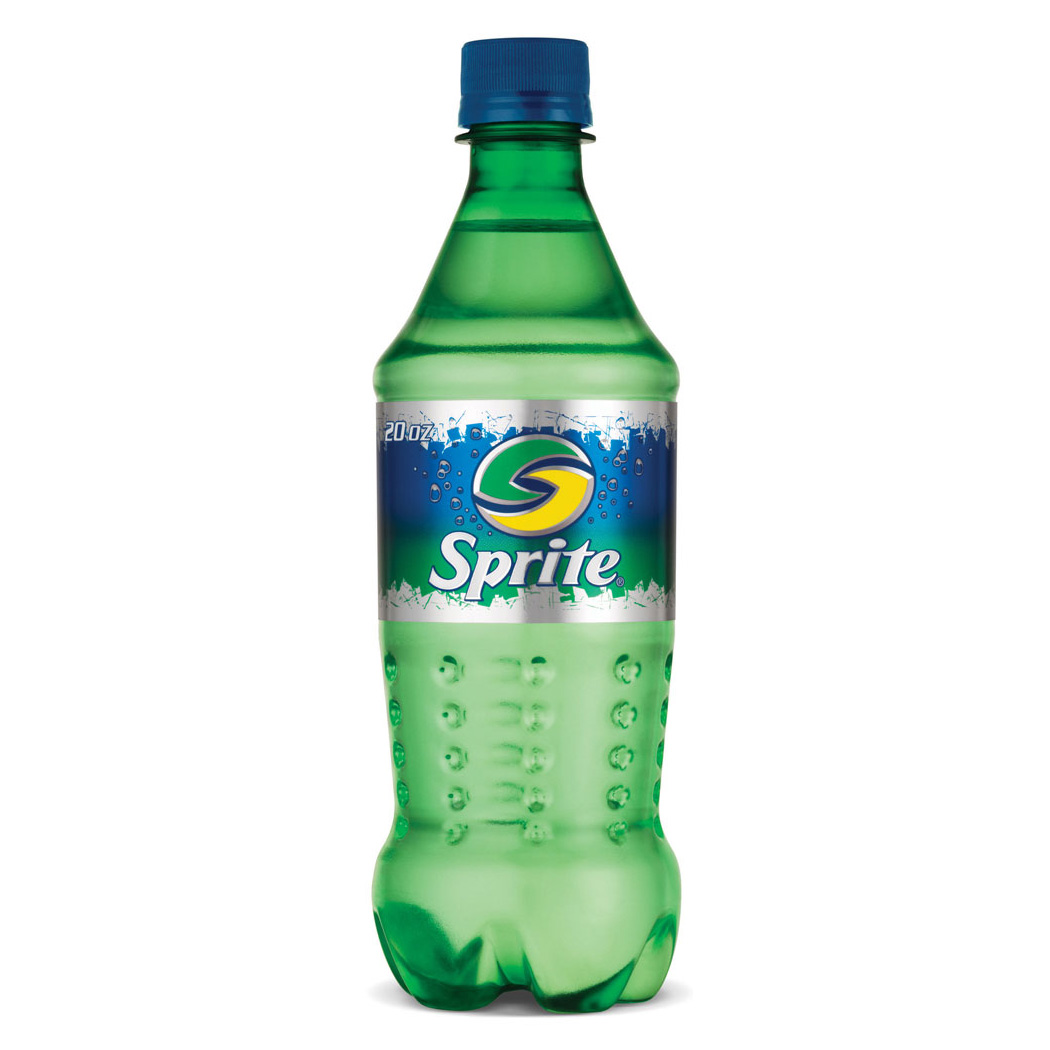
\includegraphics[scale=0.125]{sprite.jpg}
          \end{columns}
        }
        \only<3>{
          \begin{block}{Variation in the sense of \lexi{knock up}}
            \begin{itemize}
              \item `wake up' (UK)
              \item `get pregnant' (US)
            \end{itemize}
          \end{block}
        }
        \only<4>{
          \begin{block}{Variation in the sense of \lexi{pissed}}
            \begin{itemize}
              \item `drunk' (UK)
              \item `angry' (US)
            \end{itemize}
          \end{block}
        }
        \only<5>{
          \begin{block}{Stylistic variation in lexical expressions}
            If you were telling your grandmother about that time you fell:
            \begin{enumerate}
              \item \uttr{I fell on my backside.}
              \item \uttr{I fell on my ass.}
            \end{enumerate}
          \end{block}
        }
      \end{frame}

    \subsection{\suboneseven}
      \begin{frame}{\suboneseven}
        \begin{block}{Try these}
          \textcite{dawson_language_2016}, chapter 10 exercises 15, 16, and 17
        \end{block}
      \end{frame}

      \begin{frame}{References}
        \printbibliography
      \end{frame}
\end{document}
